\documentclass{resume}

\begin{document}

\fontfamily{ppl}\selectfont

\noindent
\begin{tabularx}{\linewidth}{@{}m{0.8\textwidth} m{0.2\textwidth}@{}}
{
    \Large{Akash Ramanand Rajak} \newline
    \small{
        \clink{
            \href{mailto:aakashrajak02@gmail.com}{aakashrajak02@gmail.com} \textbf{·}
            % \href{mailto:435_bt19@iiitkalyani.ac.in}{435_bt19@iiitkalyani.ac.in}
            %\newline
            {\fontdimen2\font=0.75ex +91 8980153352} 
            % \textbf{·} 
            %\href{https://johnmyweb.com}{johnmyweb.com}
        } \newline
        \clink{
        	\href{https://github.com/akash435}{Github}
        	\textbf{·} 
        	\href{https://www.linkedin.com/in/akash-rajak-akash435/}{Linkedin}\textbf{·}
        	\href{https://www.hackerrank.com/aakashrajak02?hr_r=1}{HackerRank}\textbf{·}
        	\href{https://www.codechef.com/users/akash435}{CodeChef}
        	\textbf{·}
        	\href{https://codeforces.com/profile/aakashrajak02}{Codeforces}
        	\textbf{·}
        	\href{https://leetcode.com/akash435/}{LeetCode}
            %\newline
        } \newline
        Gujarat, India
    }
} & 
{
    \hfill
    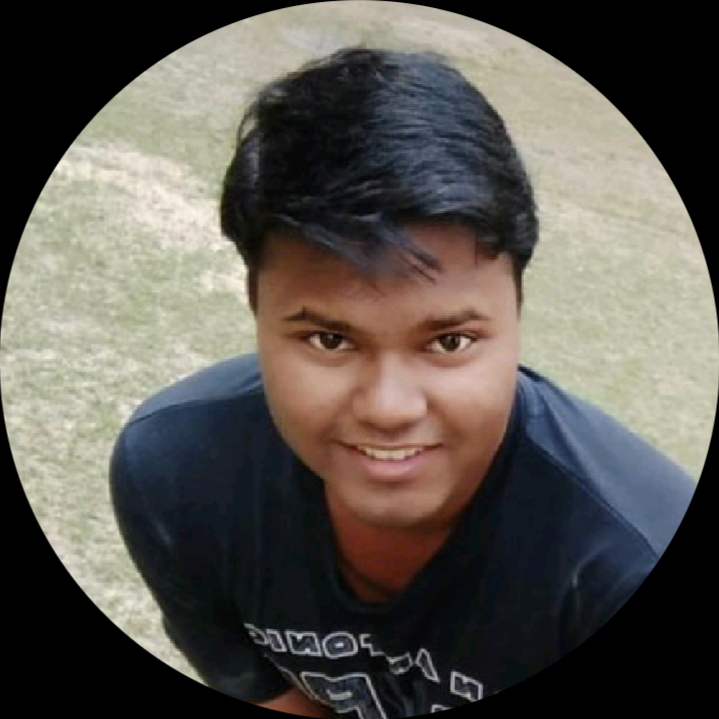
\includegraphics[width=2.8cm]{images/image1.png}
}
\end{tabularx}
\begin{center}
\begin{tabularx}{\linewidth}{@{}*{2}{X}@{}}
% left side %
{
    \csection{EXPERIENCE}{\small
        \begin{itemize}
            % item 1 %
            \item \frcontent{Student Member}{Student Member at Developer Student Club - IIIT Kalyani}{}{JAN 2021 - MAR 2021}
            % item 2 %
            % \item \frcontent{Old Dream Company}{Senior Member of Technical Staff − Texas}{Designer and implementor of a system for retrieving and caching electronic commerce content including a crawler and custom full-text indexing system that allows flexible keyword searching of product information.}{February 1999 to August 1999}
        \end{itemize}
    }
    \csection{EDUCATION}{\small
        \begin{itemize}
            % item 1 %
            \item \frcontent{HSC - Maths, Physics, Chemistry}{Baroda High School, Alkapuri}{}{2016 - 2018}
            \item \frcontent{B - Tech Computer Science}{Indian Institute of Information Technology, Kalyani}{}{2019 - 2023}
        \end{itemize}
    }
    \csection{COURSES}{\small
        \begin{itemize}
            \item \textbf{Mathematics} \newline
            {\footnotesize Probability and Statistics, Dicrete Mathematics, Linear Algebra, Calculus}{}{}
            \item \textbf{Computer Science} \newline
            {\footnotesize Programming with C, Data Structure and Algorithm, Algorithm - 1, Computer Architecture, Automata Theory}
            \item \textbf{Electronics} \newline
            {\footnotesize Digital Electronics, Analog Electronics}
        \end{itemize}
    }
    \csection{SKILLS}{\small
        \begin{itemize}
            \item \textbf{Technologies} \newline
            {\footnotesize C, C++, Java, Python, HTML, CSS, Android Development, Scilab, Qtspim}{}{}
            \item \textbf{Patterns \& Practices} \newline
            {\footnotesize Object Oriented Programming, Competitive Programming}
            \item \textbf{Languages} \newline
            {\footnotesize English, Hindi, Gujarati}
        \end{itemize}
    }
} 
% end left side %
& 
% right side %
{
    \csection{PROJECTS}{\small
        \begin{itemize}
            \item \frcontent{CaveManGame \clink{\href{https://github.com/akash435/Cave-Man-Game}{[github.com/Cave-Man-Game]}}}{- An Android based adventurous game app.}{- Used Android Studio as Frotend part and java code and Sqlite database part as backend, and developed a simple android game app.\newline - In this we get a chance to play the game of selected level, also have option to play music, can also see the highscore of each level, and many more.}{+ Features used - Java, Android, Sqlite database}
            \item \frcontent{NegativeDecimalToBinary \clink{\href{https://github.com/akash435/Negative-Decimal-to-Binary}{[github.com/NegativeDecimaltoBinary]}}}{- C Program to convert Negative Decimal No. to equivalent Binary No.}{- Tried to convert the negative decimal number and counted for the first 100 negative decimal number and displayed it in .txt file.}{+ Features used - C Language, File Handling}
            \item \frcontent{Tabular-ML \clink{\href{https://github.com/akash435/Tabular-ML}{[https://github.com/Tabular-ML]}}}{-      Built an end-to-end ML system for tabular datasets.}{ - Took a sample titanic event dataset and from the tabular dataset predicted the how many childrens,, mens, womens, captains, etc. got rescued and how many died and injured.\newline - Used the Python packages like numpy, random, pandas, seaborn, matplotlib.pyplot, etc. and we accordingly trained the data and tested also.}{+ Features used - Python, Jupiter Notebook}
        \end{itemize}
    }
    \csection{OTHER HIGHLIGHTS}{\small
        \begin{itemize}
            \item {\footnotesize Participated in Google Coding Competition - HashCode 2021, CodeJam 2021, KickStart 2021.}
            \item {\footnotesize Participated in Devfolio Hackathon HackData 5.0, with project BSM.}
        \end{itemize}
    }
    
}
\end{tabularx}
\end{center}
\end{document}\